\chapter{Análisis de resultados}

En este capítulo se presenta el análisis de los resultados obtenidos en la 
simulación por elementos finitos, tanto el caso bidimesional como el tridimensional. 
Se comparan los resultados obtenidos en ambos casos con lo obtenido de manera 
experimental mediante el uso de extensometría. Además se analizan y comparan  
los dos enfoques de análisis numérico utilizados con la finalidad de determinar 
si un análisis bidimensional es suficiente para el proceso de formado objeto 
de este proyecto, lo cual representaría un ahorro considerable de tiempo y recursos 
computacionales.\\

\section{Del análisis de elementos finitos}

\subsection{Análisis 2D}


\subsubsection{Estatus global}

Normalmente en un análisis de tipo dinámico explícito, el balance de energía juega 
un papel importante e incluso puede utilizarse como criterio de \textit{terminación}. 
Para considerar que un análisis es aceptable, la energía cinética debe representar 
menos de un 5 \% de la energía interna del modelo, de lo contrario, los efectos 
inerciales inducidos podrían afectar de manera considerable tanto la geometría 
resultante como los datos de salida. En la figura \ref{fig:energy_status_01} se observa 
que la energía cinética representa un porcentaje menor al 2\% de la energía interna, lo 
cual implica que el análisis está dentro del rango aceptable. \\

El elemento \texttt{PLANE162}, utilizado en el mallado para el análisis bidimensional, 
tiene sólo un punto de integración, lo cual le hace robusto para grandes deformaciones 
y permite un ahorro significativo de tiempo computacional, pero esto mismo les hace 
propensos a presentar modos de energía cero. Estos modos, comúnmente referidos como 
modos de Hourglass, son de naturaleza oscilatoria y tienen periodos mucho más pequeños 
que la respuesta estructural de un sistema, resultando en estados matemáticos que físicamente 
no son posibles y que normalmente tienden a deformar la malla en forma de zigzag.
Para verificar que la deformación de Hourglass no ha influido de manera considerable 
en un análisis se debe comparar la energía interna del modelo con la energía de Hourglass, 
esta última no debe ser mayor al 10\% de la primera para considerar aceptable los 
resultados de la simulación ~\cite{lsdyna-ansys-manual}. En la gráfica de la figura \ref{fig:hourglass_internal_01} 
se muestra la energía interna vs la energía de Hourglass y se aprecia que la proporción 
varía en un rango del 1.5 a 2\%, lo cual indica que la deformación de Hourglass se encuentra 
dentro de los límites aceptables.

\begin{center}
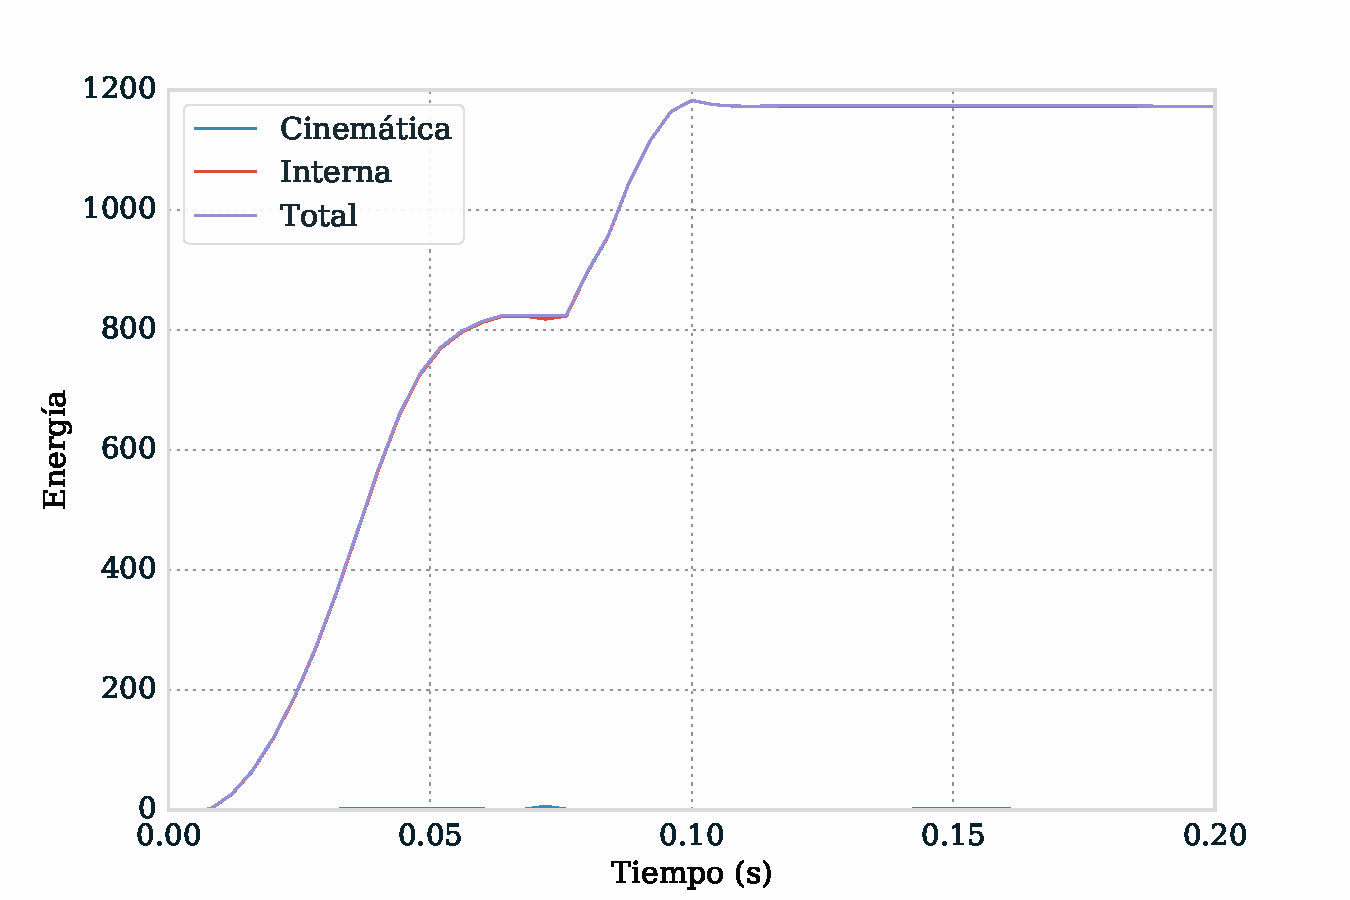
\includegraphics[width=0.8\textwidth]{src/ch4/energy_status_01.pdf}
\captionof{figure}{Variación de la energía total, interna y cinemática, primer paso}
\label{fig:energy_status_01}
\end{center}


\begin{center}
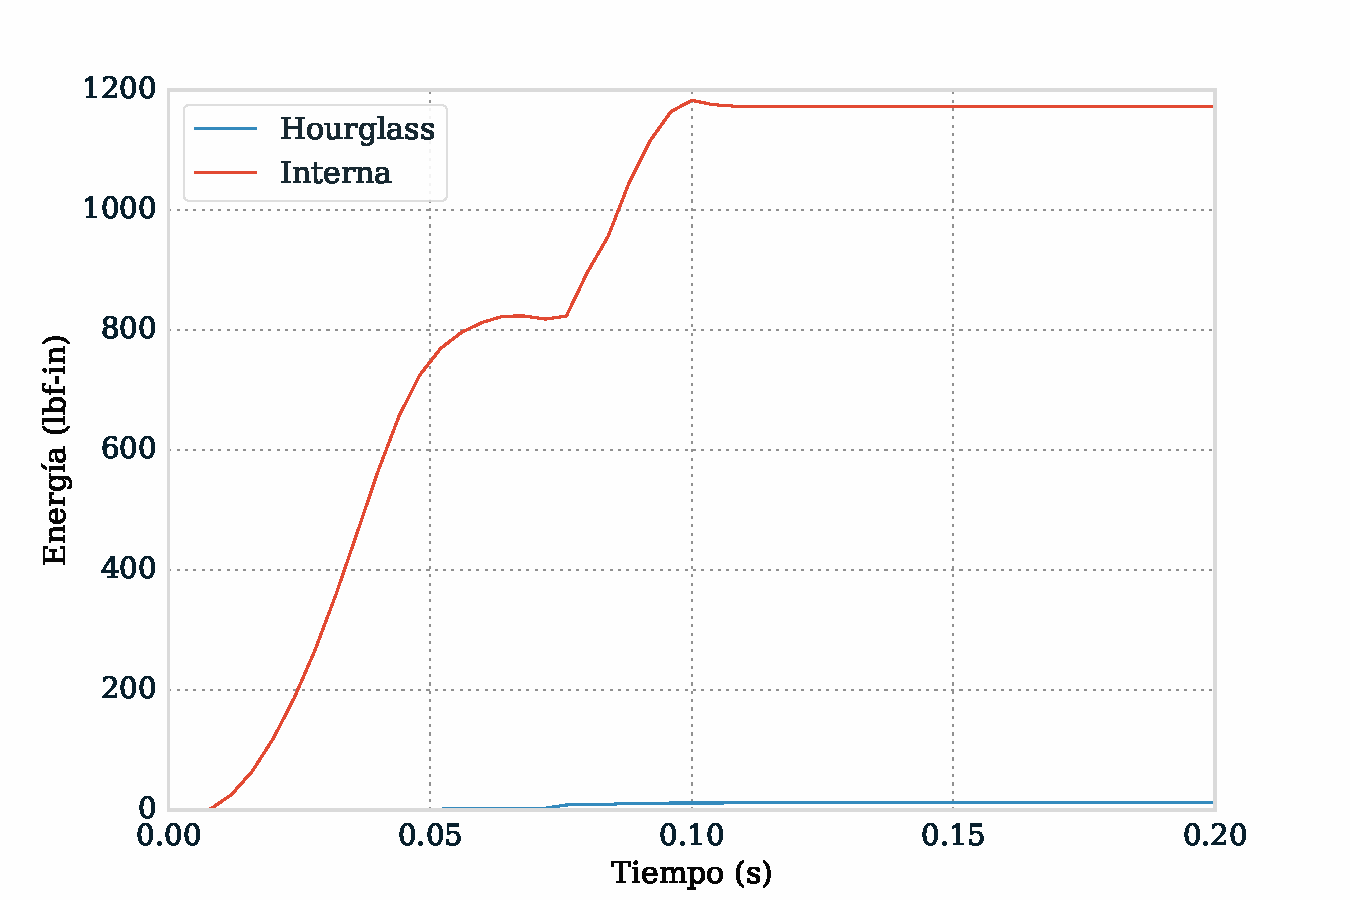
\includegraphics[width=0.8\textwidth]{src/ch4/hourglass_internal_01.pdf}
\captionof{figure}{Comparación energía interna vs energía de Hourglass}
\label{fig:hourglass_internal_01}
\end{center}


\subsubsection{Geometría resultante}

En la figura \ref{fig:shape_sequence_01} se muestra la secuencia de formado 
de la geometría resultante, se puede apreciar el doblado en U y el doblado 
llevado a cabo por las levas.

\begin{center}
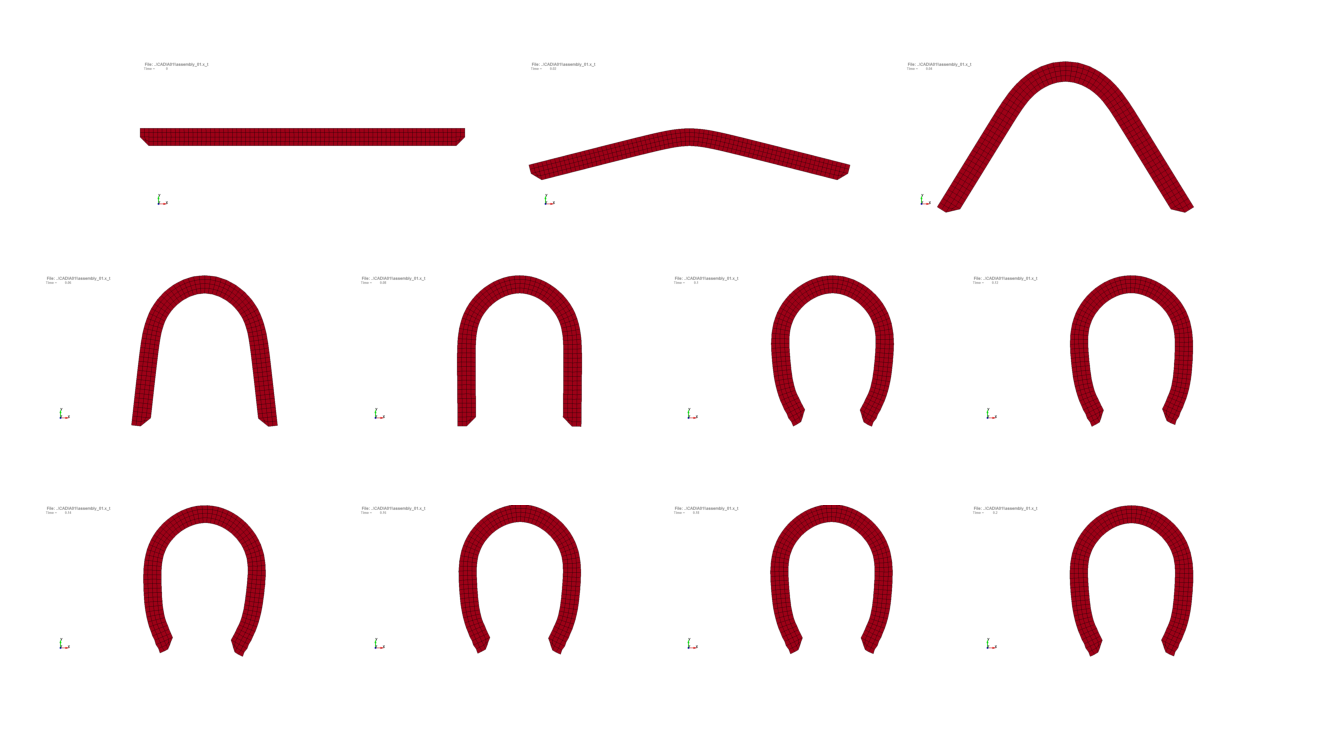
\includegraphics[width=0.95\textwidth]{src/ch4/shape_sequence_01.pdf}
\captionof{figure}{Secuencia de la geometría resultante}
\label{fig:shape_sequence_01}
\end{center}

Las figuras \ref{fig:geometry_01} y \ref{fig:geometry_02} muestran las geometrías 
resultantes al final del primer y segundo paso del proceso de formado.

\begin{center}
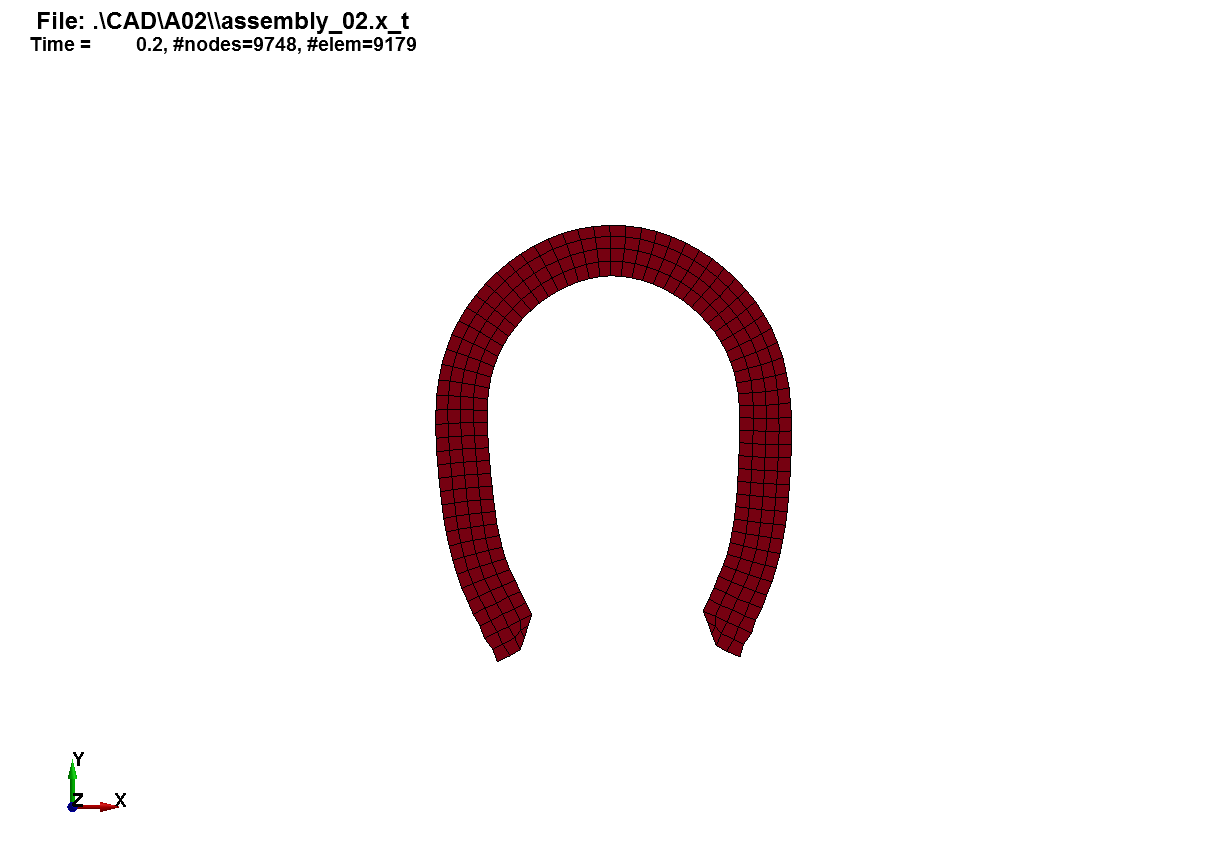
\includegraphics[width=0.75\textwidth]{src/ch4/geometry_01.png}
\captionof{figure}{Geometría resultante, primer paso}
\label{fig:geometry_01}
\end{center}

\begin{center}
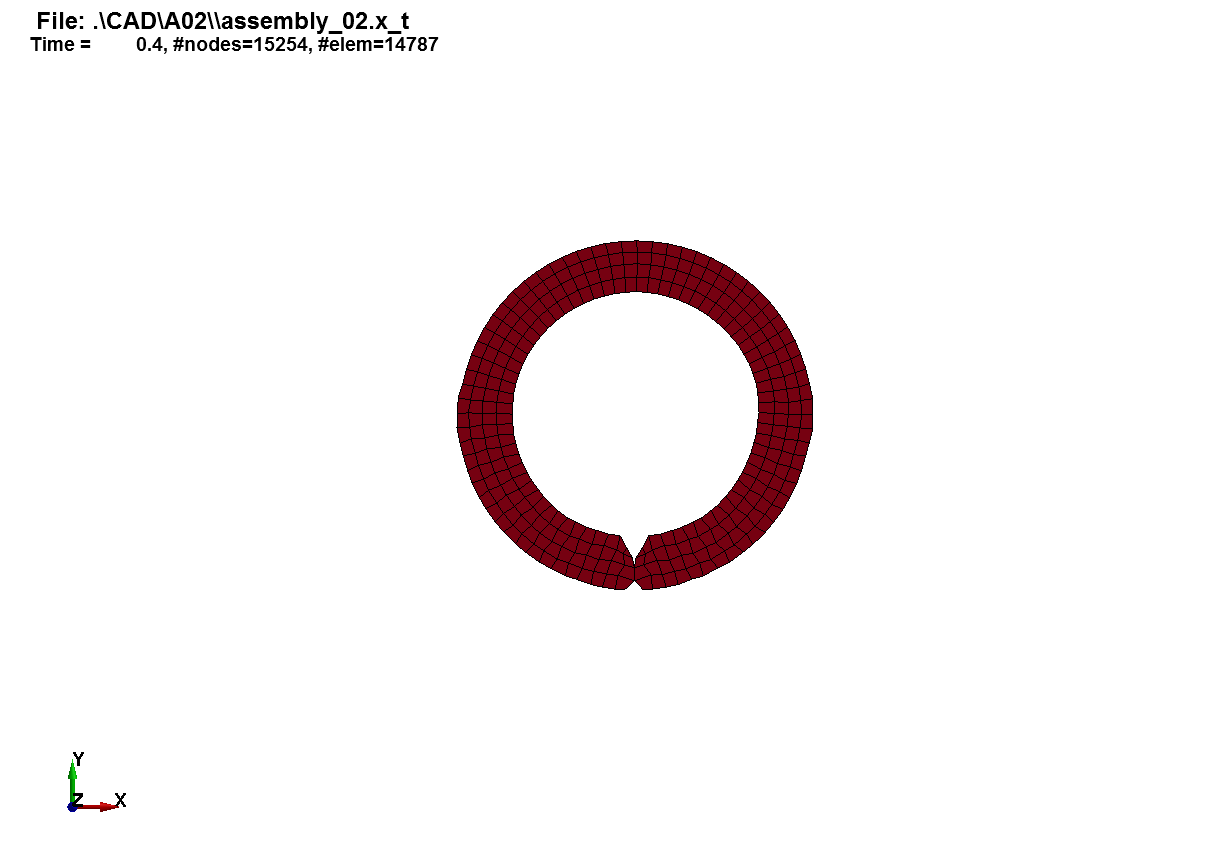
\includegraphics[width=0.75\textwidth]{src/ch4/geometry_02.png}
\captionof{figure}{Geometría resultante, segundo paso}
\label{fig:geometry_02}
\end{center}

En la figura \ref{fig:thickness_variation} se muestra una gráfica con las variaciones de espesor en la geometría final obtenida, las líneas punteadas corresponden a las tolerancias mínima y máxima del espesor. Para efectuar tal medición se tomaron como referencia nodos interiores y exteriores en la geometría final, posicionados sobre la misma vertical en la geometría inicial, y enseguida, basándose en las coordenadas iniciales y los desplazamientos, se obtuvo la distancia.

\begin{center}
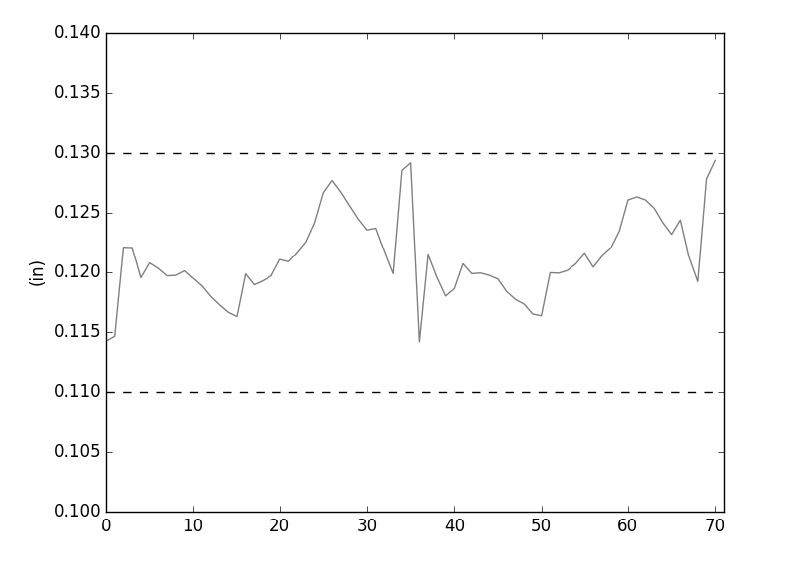
\includegraphics[width=0.85\textwidth]{src/ch4/thickness_variation.png}
\captionof{figure}{Variación del espesor de la geometría resultante}
\label{fig:thickness_variation}
\end{center}



\subsubsection{Esfuerzos}

\begin{center}
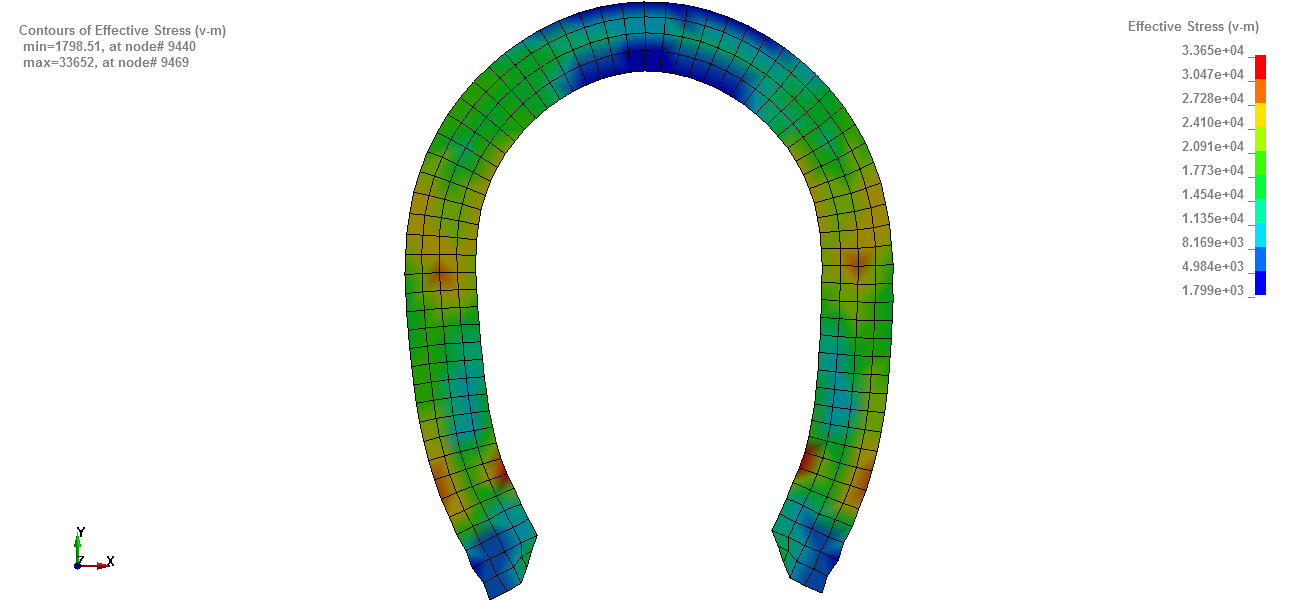
\includegraphics[width=0.75\textwidth]{src/ch4/von_mises_01.png}
\captionof{figure}{Distribución de esfuerzos de von Mises, final del primer paso}
\label{fig:von_mises_01}
\end{center}

\begin{center}
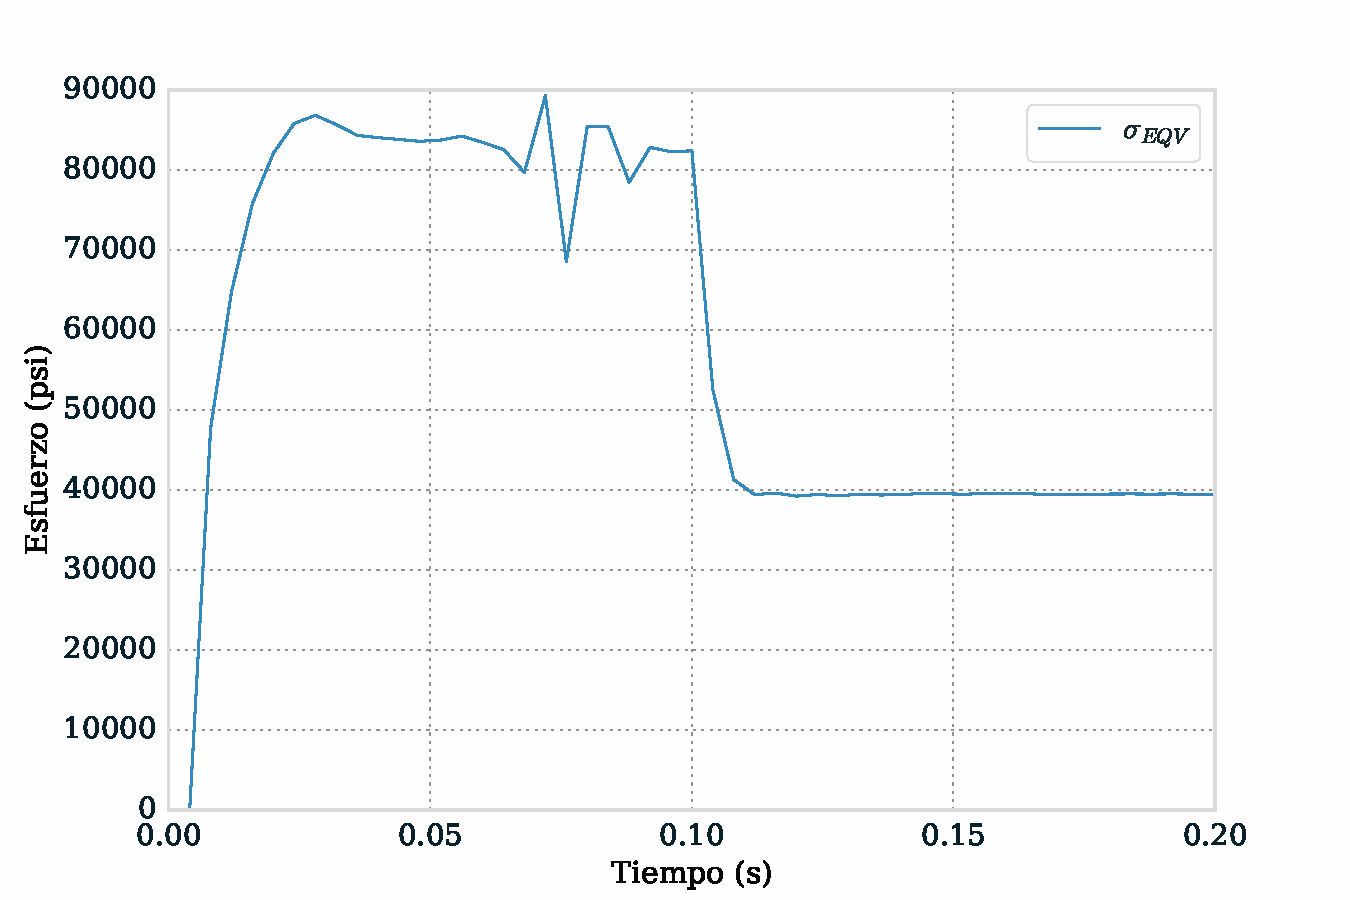
\includegraphics[width=0.75\textwidth]{src/ch4/von_mises_stress_01.pdf}
\captionof{figure}{Variación del esfuerzo máximo de von Mises}
\label{fig:von_mises_stress_01}
\end{center}

\begin{center}
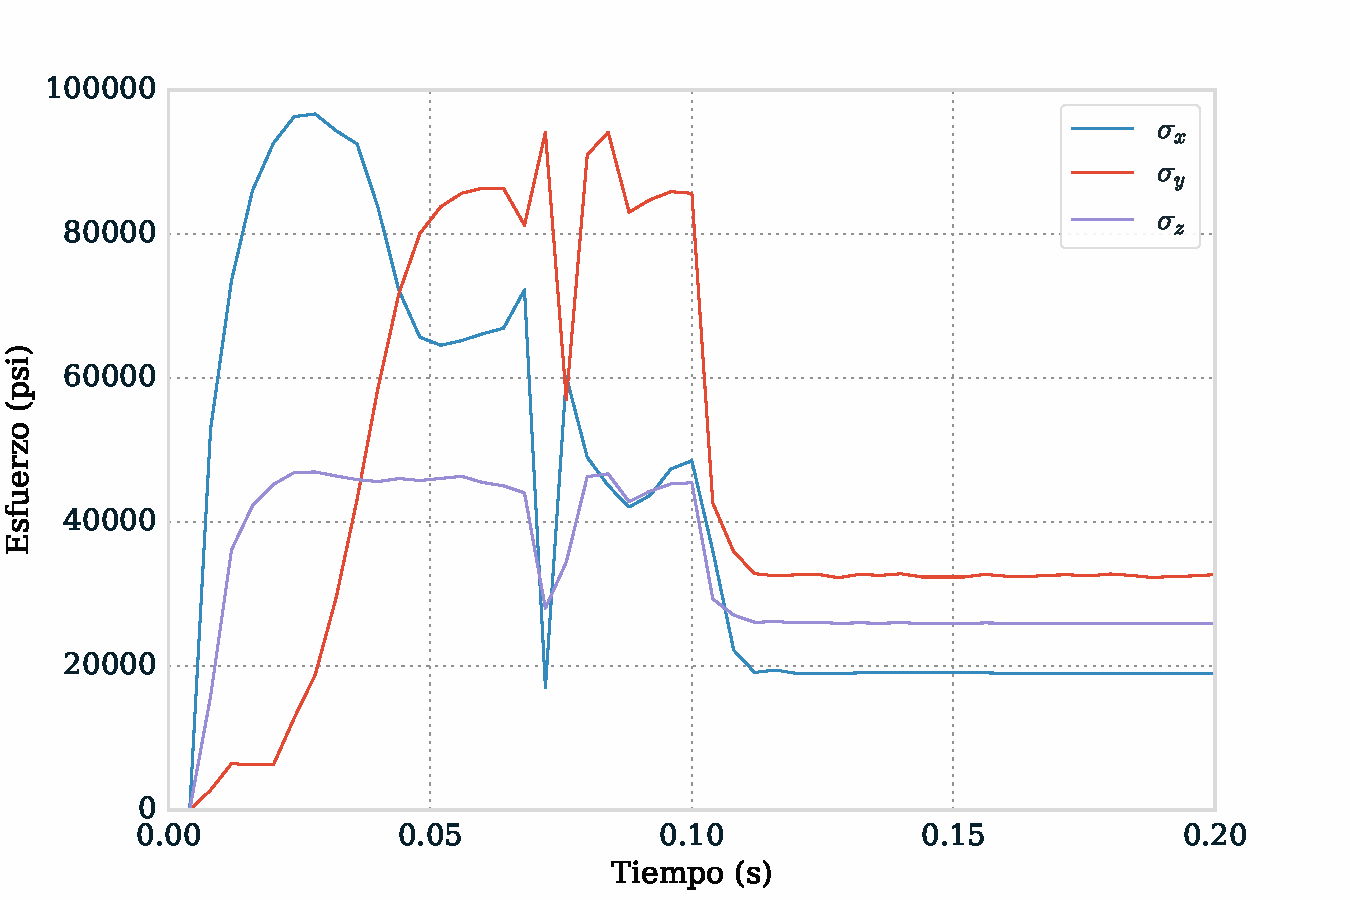
\includegraphics[width=0.75\textwidth]{src/ch4/xyz_stress_01.pdf}
\captionof{figure}{Variación de los esfuerzos máximos en dirección X,Y,Z}
\label{fig:xyz_stress_01}
\end{center}

\begin{center}
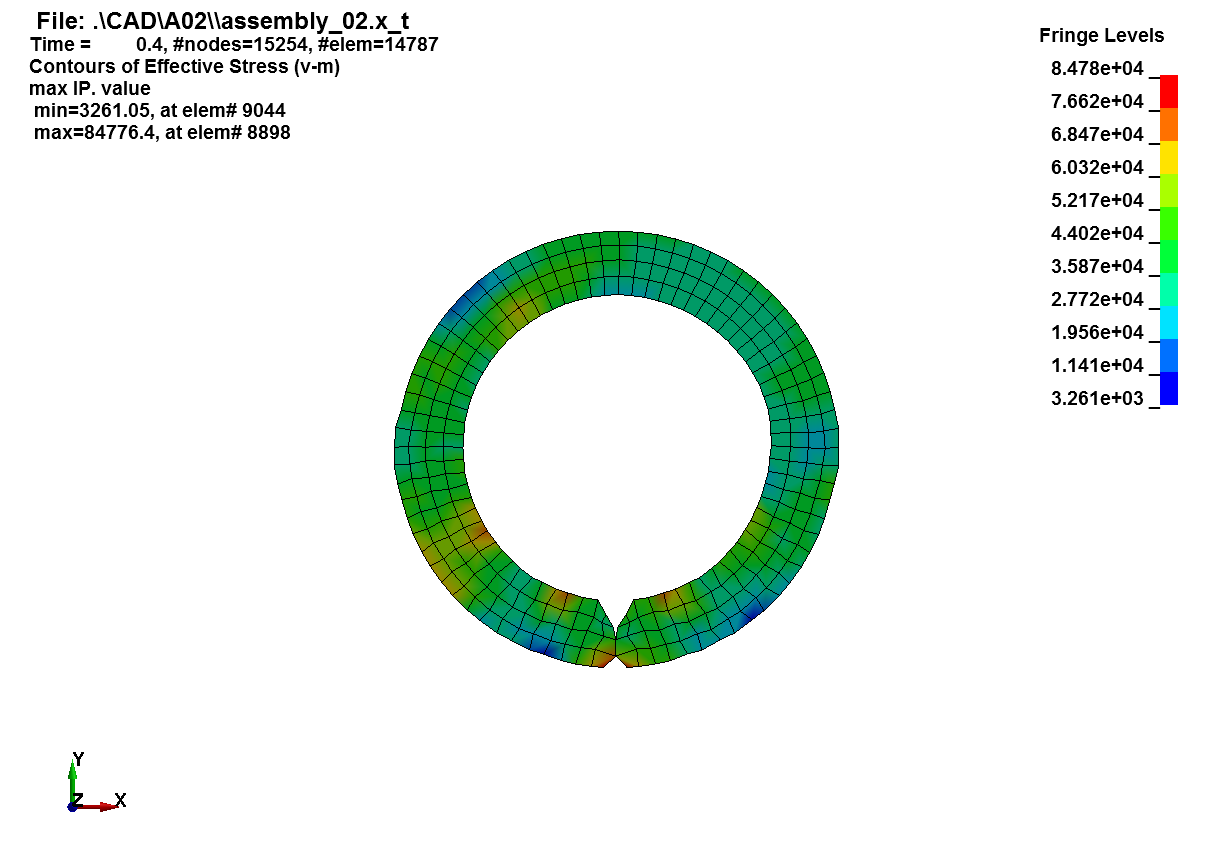
\includegraphics[width=0.75\textwidth]{src/ch4/von_mises_02.png}
\captionof{figure}{Distribución de esfuerzos de von Mises, final del segundo paso}
\label{fig:von_mises_01}
\end{center}


\subsubsection{Deformaciones}

\begin{center}
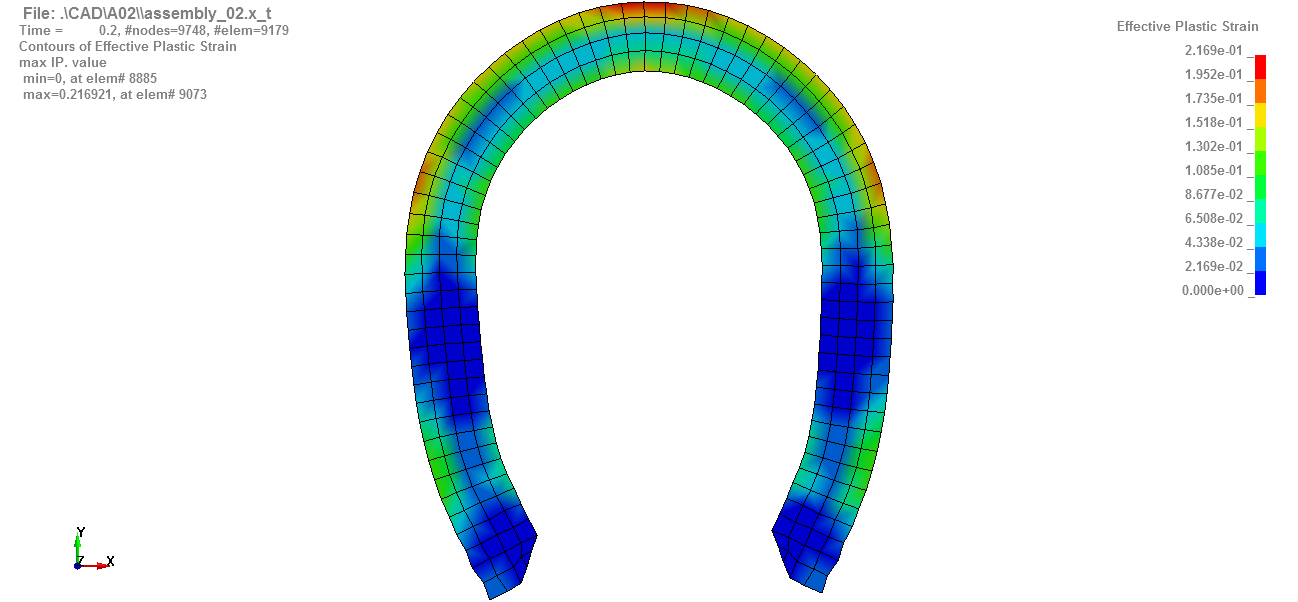
\includegraphics[width=0.75\textwidth]{src/ch4/efective_plastic_strain_01.png}
\captionof{figure}{Deformación plástica efectiva, final del primer paso}
\label{fig:efective_plastic_strain}
\end{center}

\begin{center}
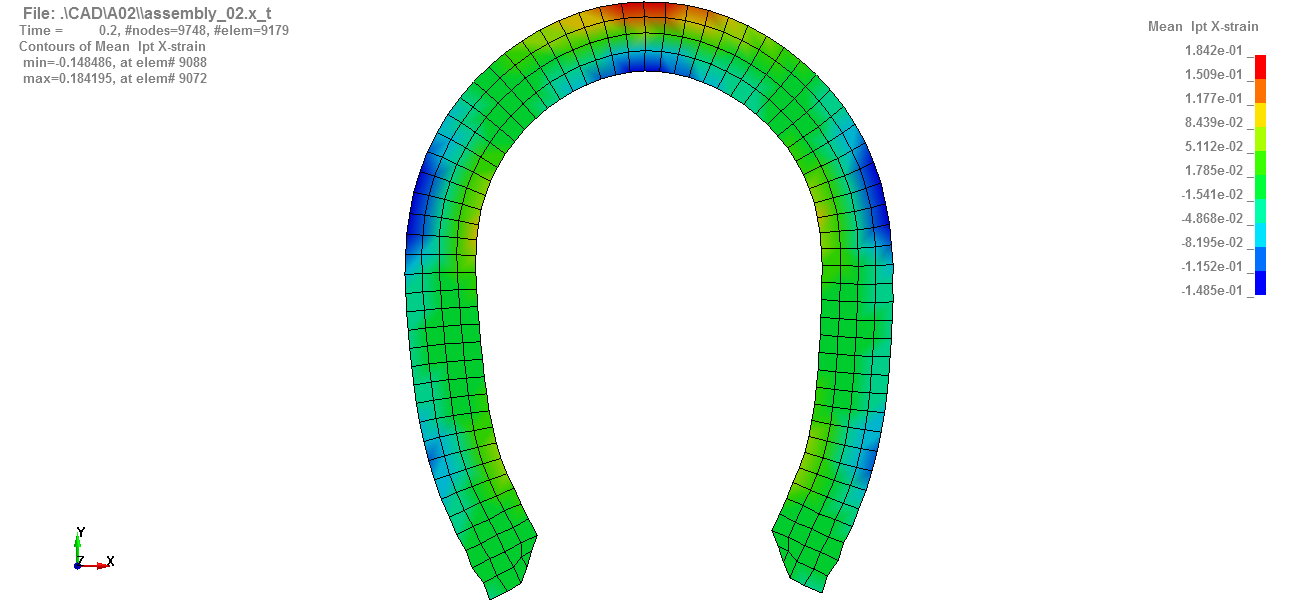
\includegraphics[width=0.75\textwidth]{src/ch4/strain_x_01.png}
\captionof{figure}{Deformación en dirección X, final del primer paso}
\label{fig:efective_plastic_strain}
\end{center}

\begin{center}
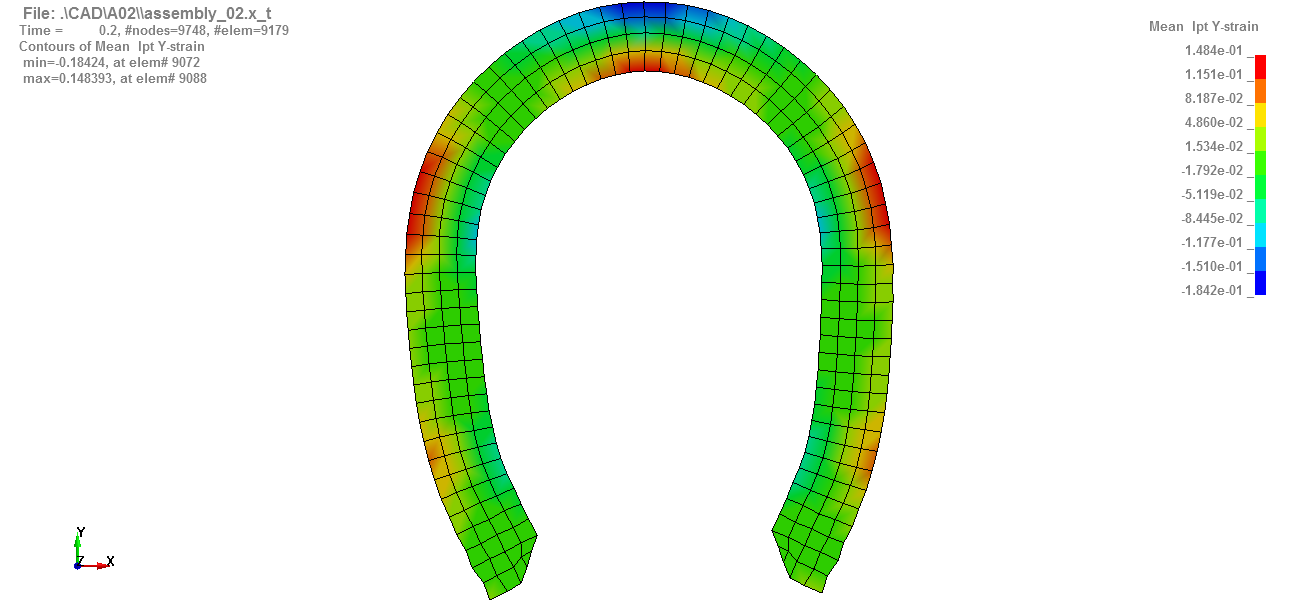
\includegraphics[width=0.75\textwidth]{src/ch4/strain_y_01.png}
\captionof{figure}{Deformación en dirección Y, final del primer paso}
\label{fig:efective_plastic_strain}
\end{center}


\begin{center}
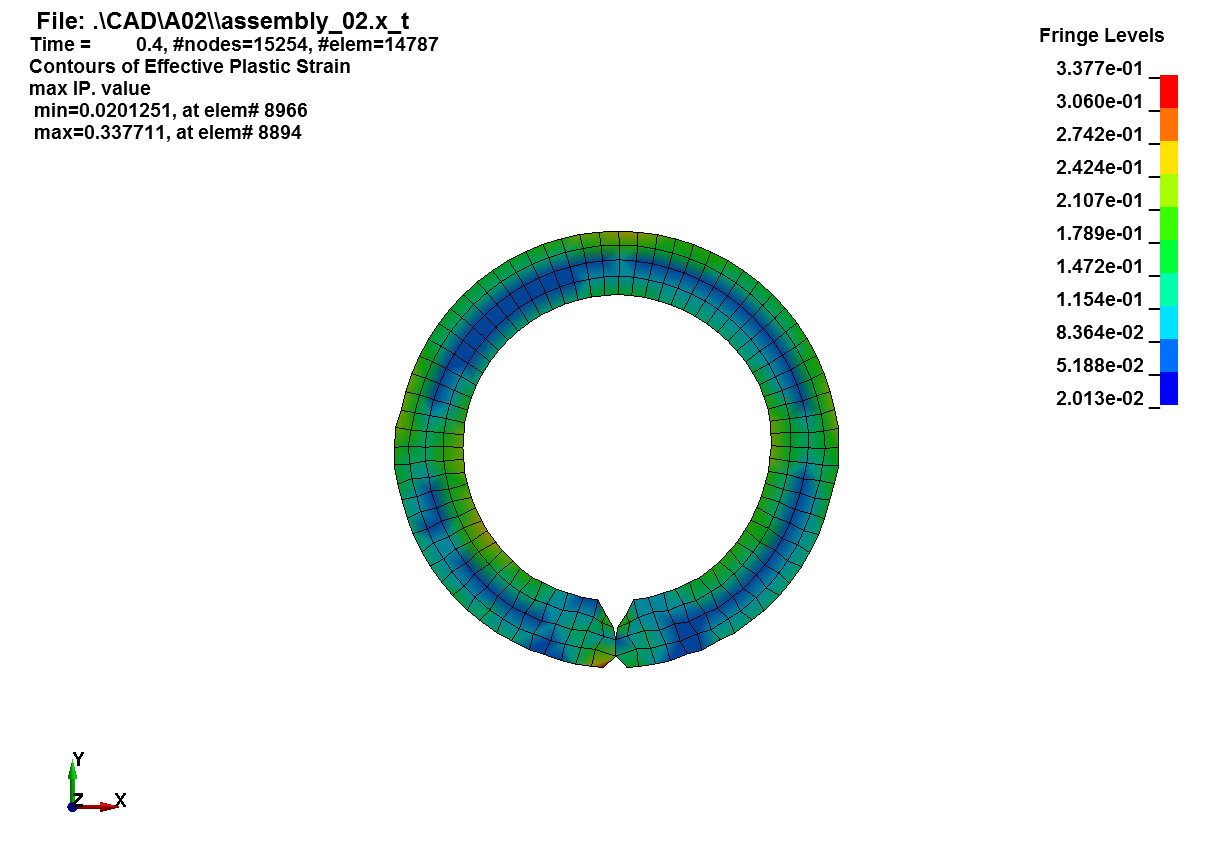
\includegraphics[width=0.75\textwidth]{src/ch4/efective_plastic_strain_02.png}
\captionof{figure}{Deformación plástica efectiva, final del segundo paso}
\label{fig:efective_plastic_strain}
\end{center}

\begin{center}
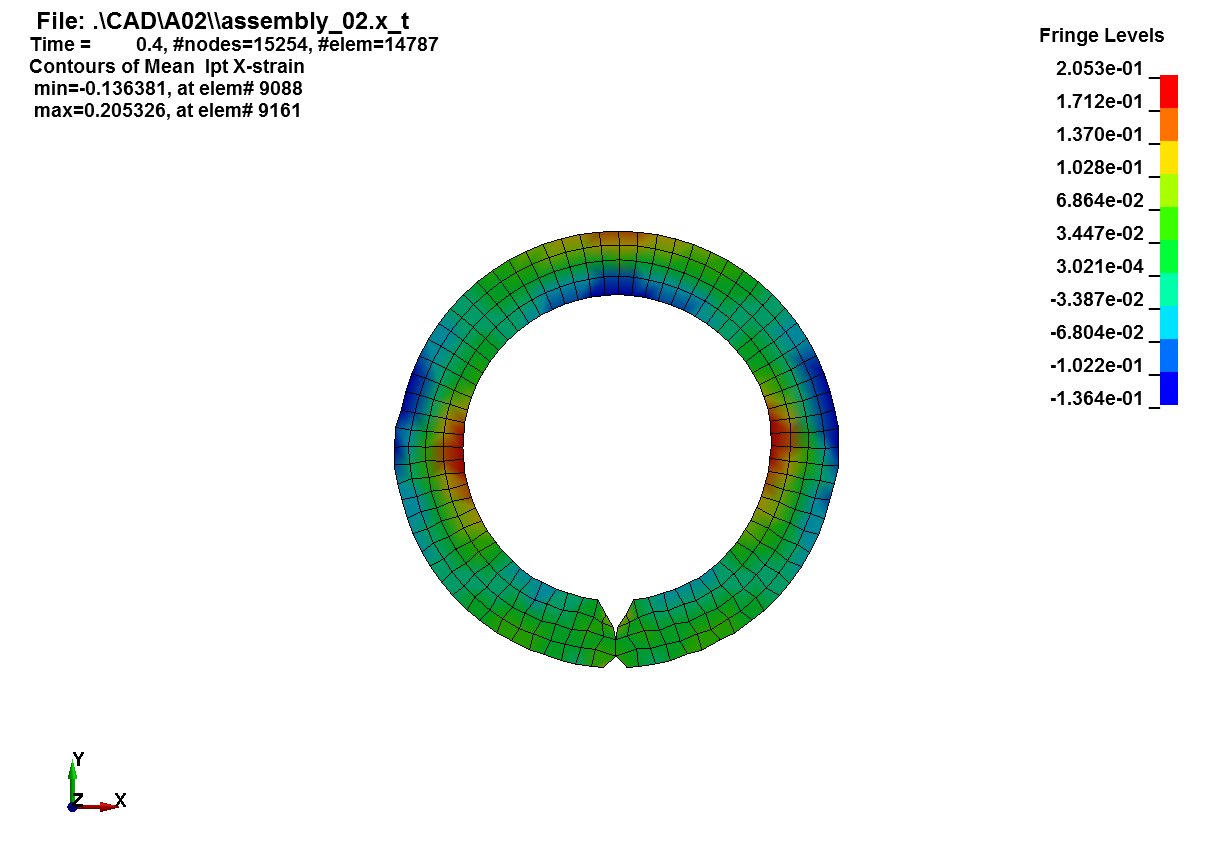
\includegraphics[width=0.75\textwidth]{src/ch4/strain_x_02.png}
\captionof{figure}{Deformación en dirección X, final del segundo paso}
\label{fig:efective_plastic_strain}
\end{center}

\begin{center}
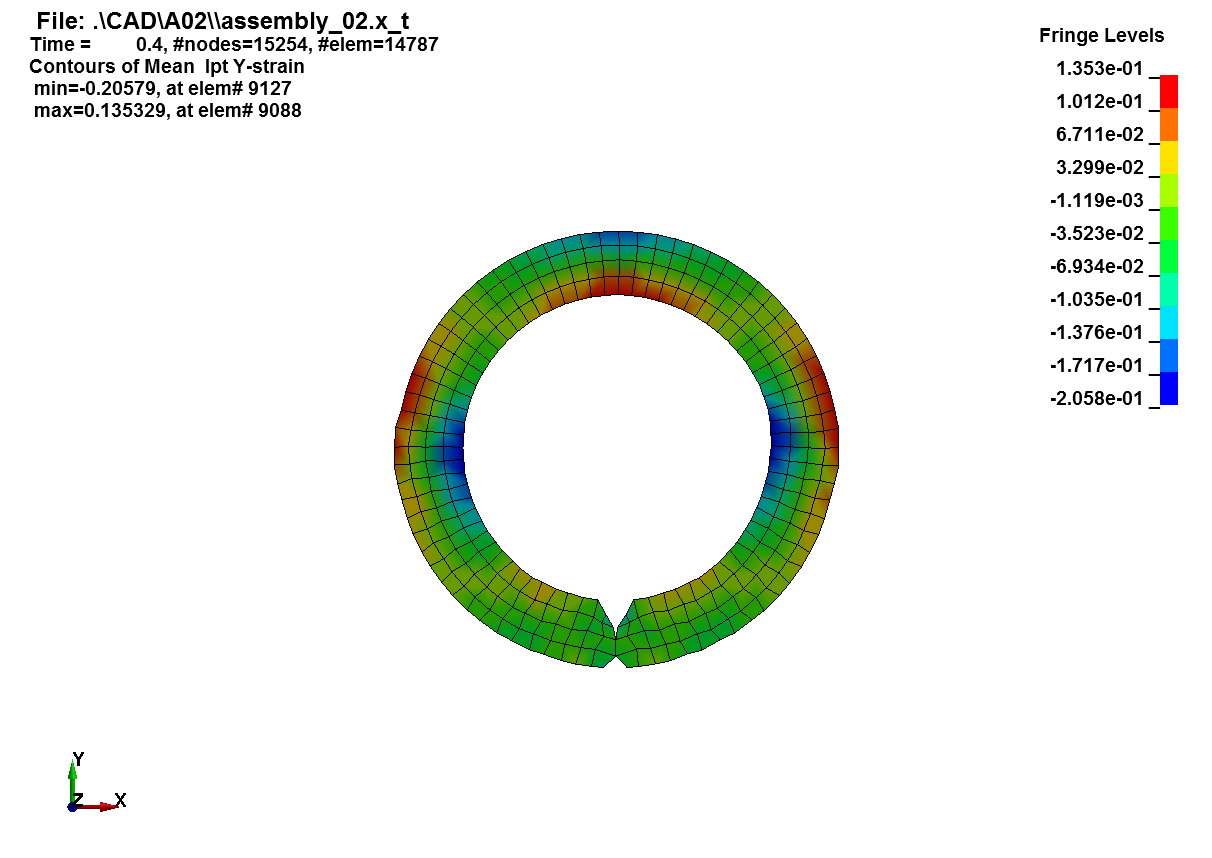
\includegraphics[width=0.75\textwidth]{src/ch4/strain_y_02.png}
\captionof{figure}{Deformación en dirección Y, final del segundo paso}
\label{fig:efective_plastic_strain}
\end{center}



\subsection{Análisis 3D}


\subsubsection{Estatus global}

\begin{center}
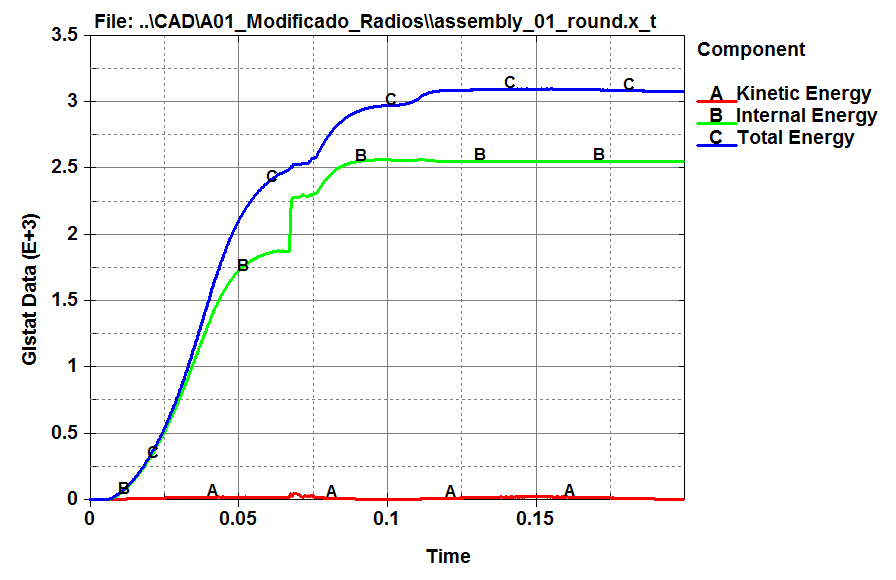
\includegraphics[width=0.75\textwidth]{src/ch4/energy_status_3d.png}
\captionof{figure}{Energía interna, cinética y total}
\label{fig:von_mises_3D_01}
\end{center}

\subsubsection{Esfuerzos}


\begin{center}
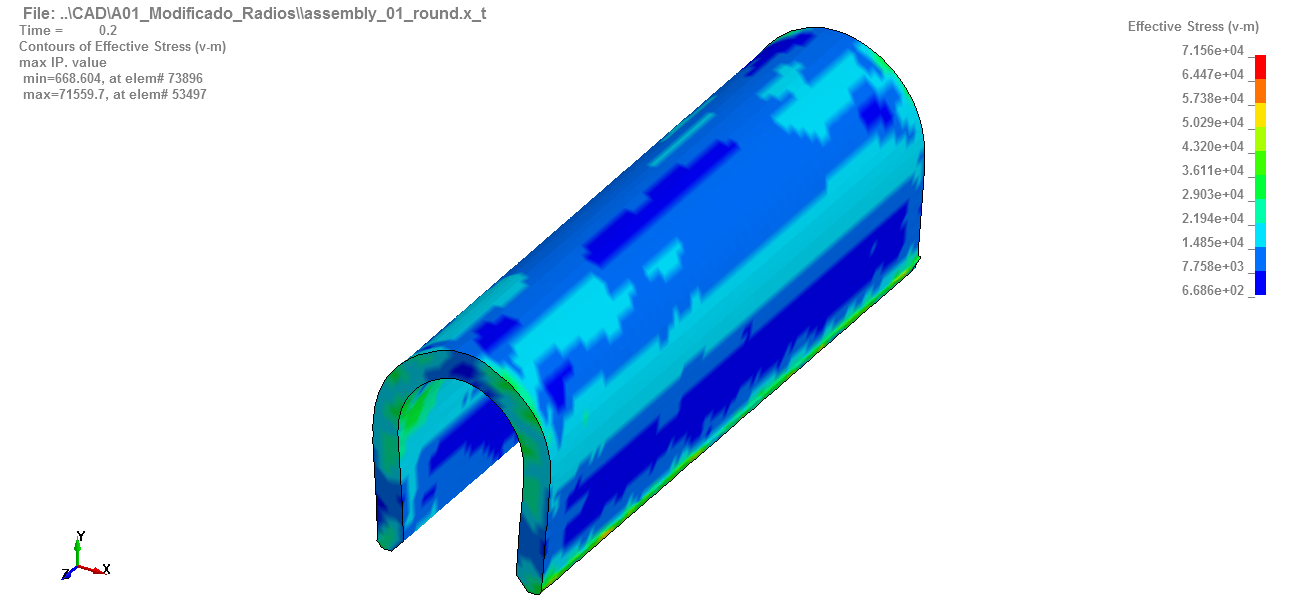
\includegraphics[width=0.75\textwidth]{src/ch4/von_mises_3D_01.png}
\captionof{figure}{Distribución del esfuerzo de von Mises}
\label{fig:von_mises_3D_01}
\end{center}

\begin{center}
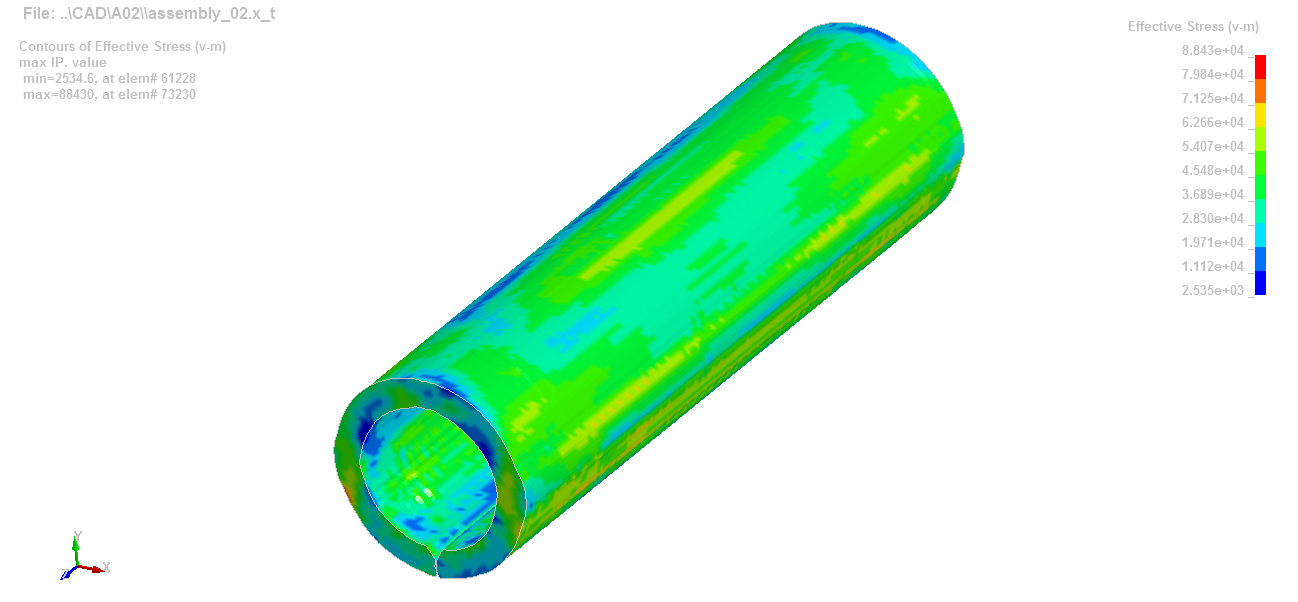
\includegraphics[width=0.75\textwidth]{src/ch4/von_mises_3D_02.png}
\captionof{figure}{Distribución del esfuerzo de von Mises, segundo paso}
\label{fig:von_mises_3D_02}
\end{center}

\subsubsection{Deformaciones}

\begin{center}
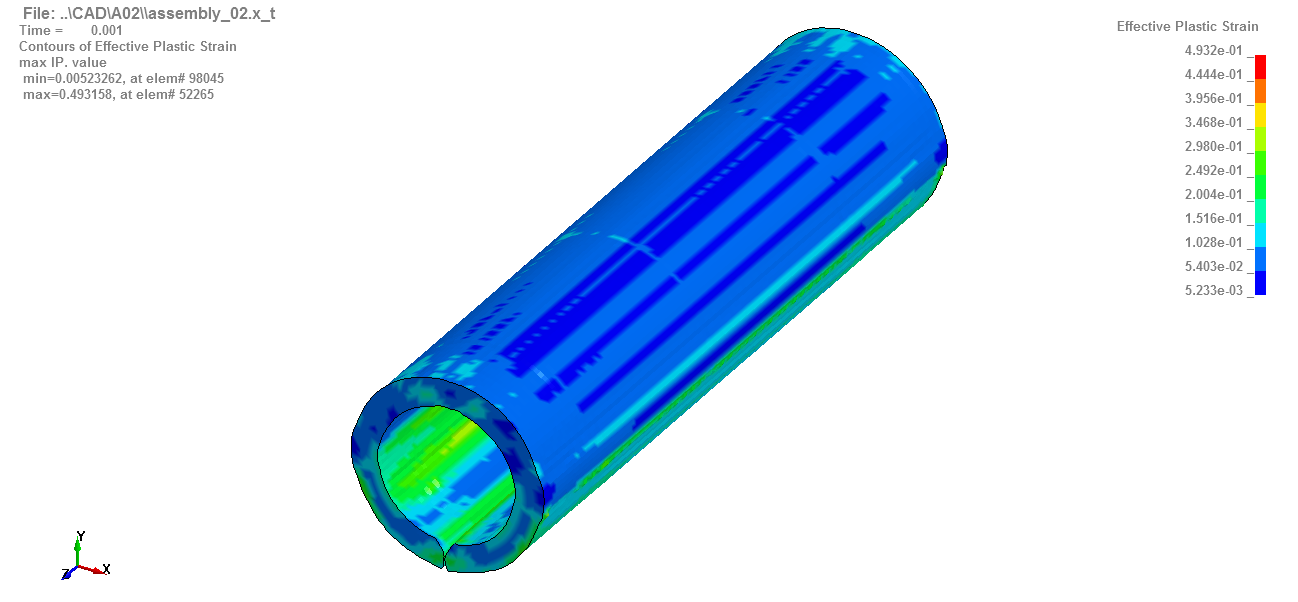
\includegraphics[width=0.75\textwidth]{src/ch4/eqv_strain_01.png}
\captionof{figure}{Deformación plástica equivalente, primer paso}
\label{fig:eqv_strain_01}
\end{center}


\subsection{Comparación 2D vs 3D}

En esta sección se presenta un análisis comparativo entre el análisis bidimensional 
y el análisis en tres dimensiones.

\subsubsection{Tiempo de cómputo}

\subsubsection{Fuerza de formado}


\section{Del análisis experimental}


